\section{Results and Discussion}
\label{sec:results}

\policytable{tables/policy_C.tex}{Selection policies with the same number of node updates, all on the same weights. $F_{\mathrm{pres}}$: event preservation against the full-update model's own detections. $R^{\mathrm{adv}}_{\mathrm{pres}}$: share of the full model's adventitious detections that are preserved. $F$ and seg-adv-$F$: scores against the annotations. Bold: best policy per column and budget, excluding the hindsight oracle and the w/o-refresh ablation. $^\dagger$Hindsight oracle (runs the full update every step; not deployable). Mean$\pm$sd over three seeds.}{tab:policy}

\begin{figure}[H]
\begin{adjustwidth}{-\extralength}{0cm}
\centering
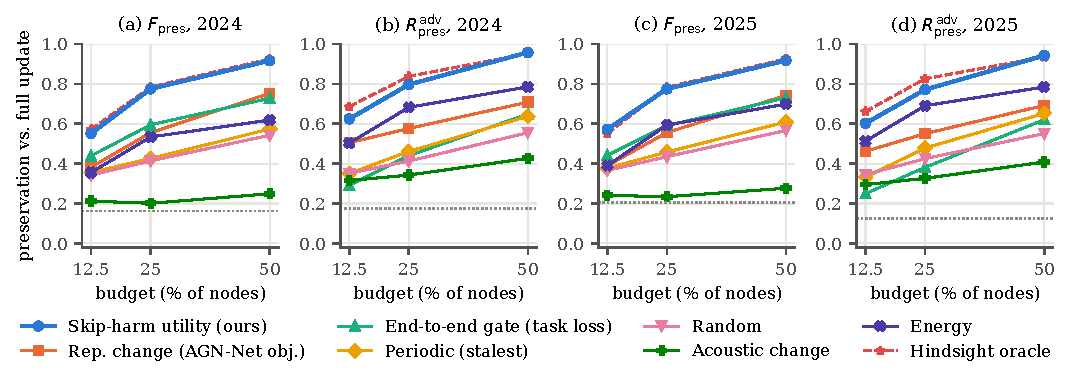
\includegraphics[width=\linewidth]{figures/budget_C.pdf}
\end{adjustwidth}
\caption{Preservation versus update budget (mean over seeds): (a) event preservation $F_{\mathrm{pres}}$, 2024 test set; (b) adventitious preservation $R^{\mathrm{adv}}_{\mathrm{pres}}$, 2024; (c) $F_{\mathrm{pres}}$, 2025 release; (d) $R^{\mathrm{adv}}_{\mathrm{pres}}$, 2025. The dotted line is the cheap path with no graph updates. Our skip-harm controller (blue) is above every non-utility baseline at every budget and close to the hindsight oracle (dashed). The hold-only variant, omitted here, lies close to ours; the label-free variant lies between ours and the change objective at 12.5\% and 25\% (Table~\ref{tab:policy}).}
\label{fig:budget}
\end{figure}

\subsection{Which Updates Can Be Skipped? (RQ1)}
Table~\ref{tab:policy} and Figure~\ref{fig:budget} compare the selection policies. Skipping matters: with no graph updates at all, event preservation drops to $F_{\mathrm{pres}}=0.163$, so the persistent state carries much of the information.

The skip-harm controller is the best deployable policy. With 25\% of the updates on the 2024 test set, it preserves the full model's events with $F_{\mathrm{pres}}=0.775$. AGN-Net's change objective reaches 0.555, energy 0.534, periodic refresh 0.425 and random selection 0.414. Our controller is close to the hindsight oracle (0.784). The gain is positive in every seed, by 0.14--0.60 over random and 0.11--0.41 over the change objective. The patient-level bootstrap gives 0.311 [0.304, 0.319] and 0.197 [0.189, 0.204], respectively ($p<0.001$). The same ordering holds at 12.5\% (0.552 vs.\ 0.382 and 0.342) and at 50\% (0.917 vs.\ 0.752 and 0.542). It also holds on the 2025 release (0.775 vs.\ 0.556 and 0.435 at 25\%) and for adventitious detections ($R^{\mathrm{adv}}_{\mathrm{pres}}=0.797$ vs.\ 0.576 and 0.413). Note that these are the model's own adventitious detections, few of which match an annotated adventitious event under the shifted annotation style.

\paragraph*{Comparison with end-to-end training} The gate trained end to end on the task loss is a competitive baseline, but it does not reach the two-stage controller. At 25\%, it preserves $F_{\mathrm{pres}}=0.595$ against 0.775 for our controller (bootstrap difference 0.212 [0.202, 0.222]), and our controller is better in every seed at every budget, by 0.07--0.35 at 25\%. On average the end-to-end gate is only slightly better than the change objective (0.555), and not in every seed. For the graph-GRU cell its results also vary strongly between seeds (Section~\ref{sec:gg}). Section~\ref{sec:why-two-stage} analyses why.

\paragraph*{Accuracy against the annotations}
Better preservation than the heuristic baselines also gives better detection, with one exception. The end-to-end gate, which preserves far fewer of the full model's events, scores slightly higher than our controller against the annotations at 25\% on the 2024 set (event $F$ 0.098; difference to ours \ensuremath{-}0.0056 [\ensuremath{-}0.0090, \ensuremath{-}0.0023]) and at 12.5\% on the 2025 release (\ensuremath{-}0.0032 [\ensuremath{-}0.0061, \ensuremath{-}0.0003]), whereas at 25\% on the 2025 release the two do not differ (0.0002 [\ensuremath{-}0.0026, 0.0034]) and at 50\% our controller is higher (0.0072 [0.0044, 0.0099]). Training directly on the task loss can thus trade fidelity to the full model for agreement with the shifted annotations. At 25\%, event $F$ against the annotations is 0.090 for our controller and 0.092 with full updates. Random and periodic selection change it by \ensuremath{-}0.046 and \ensuremath{-}0.044 (bootstrap estimates on pooled counts). For our controller the difference to full updating is \ensuremath{-}0.0026 [\ensuremath{-}0.0049, \ensuremath{-}0.0001]. Its lower bound is above the $-0.01$ margin, so selective inference with a quarter of the updates is non-inferior to full updating. The same holds on the 2025 release (\ensuremath{-}0.0002 [\ensuremath{-}0.0023, 0.0017]) and at 50\%. At 12.5\% the loss (\ensuremath{-}0.0235) exceeds the margin, although it is half that of random selection.

\paragraph*{Boundary-tolerant metrics} The low absolute event $F$ is largely a matter of boundary conventions. Table~\ref{tab:tolerant} relaxes the matching criterion. For the full-update model on the 2024 test set, event $F$ rises from 0.092 with 0.2\,s collars to 0.308 with 1\,s collars and 0.633 under overlap matching, and the 1\,s segment-based $F$ over all classes is 0.835. In preservation, our controller at 25\% is ahead of the end-to-end gate, the change objective and random selection under every criterion (e.g., overlap-based preservation 0.909 vs.\ 0.819, 0.809 and 0.738). Against the annotations, it matches full updating and is ahead of the change objective and random selection under every event-based criterion, while the end-to-end gate is slightly higher under every event-based criterion (but lower in adventitious segment $F$); segment-based scores over all classes, which are dominated by the frequent normal class, are similar for all policies.

\toltable

\diagtable

\subsection{Why Does It Work? (RQ2)}
Table~\ref{tab:diag} measures how well each scorer ranks the 64 regions by their measured skip-harm utility. The skip-harm controller reaches a Spearman correlation of 0.628 and finds 73.6\% of the true top-25\% regions (random: 24.9\%). The change-trained head, with the same architecture and inputs, reaches only 0.351. Acoustic change is even negatively correlated with utility (\ensuremath{-}0.214). This explains its ranking in Table~\ref{tab:policy}: it is the worst policy at every budget, well below random. Large spectral change is not a sign of an important update.

Utility is also concentrated in a few regions. The top 25\% of regions carry 82.4\% of the total utility but only 44.6\% of the representation change. Because the KL-based utility grows roughly quadratically, we also compare on matched scales. The top quarter still carries 65.7\% of the square-root utility against 44.6\% of the change. This concentration is what makes small budgets work: the updates that matter are few, even though the representation changes almost everywhere. Figure~\ref{fig:example} shows an example. Utility concentrates in the lower-frequency regions, which our controller updates persistently, while the change-trained controller spreads its updates widely.

\begin{figure}[H]
\centering
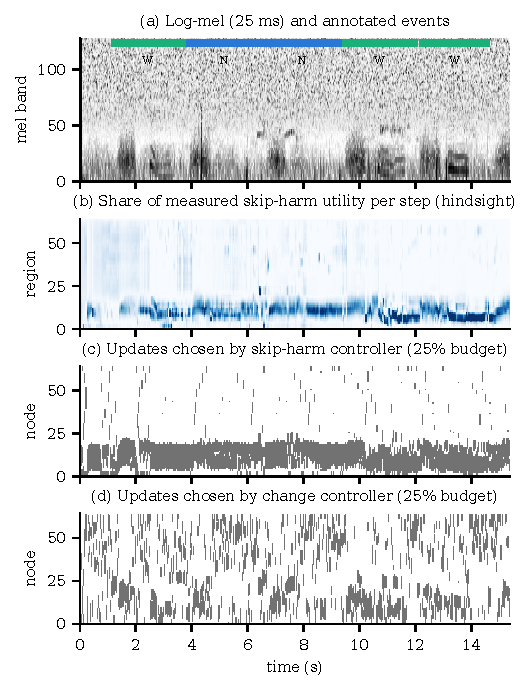
\includegraphics[width=0.72\textwidth]{figures/example.pdf}
\caption{Example 2024 test recording at a 25\% budget (seed 0). (a) Log-mel spectrogram with the annotated events (bars; W: wheeze, N: normal). (b) Each region's share of the measured skip-harm utility per step. (c) Nodes updated (dark) by our controller. (d) Nodes updated by the change-trained controller.}
\label{fig:example}
\end{figure}

\paragraph*{Why does our end-to-end gate fall short?}
\label{sec:why-two-stage}
Three observations explain the gap to the end-to-end gate in preservation. First, its training signal is weak, or at least hard to exploit with the straight-through estimator we used. The task loss of the end-to-end gate does not decrease during training (mean 1.220 in the first epoch and 1.262 in the last; 1.208 and 1.368 for the graph GRU), although the Gumbel noise is annealed (for the graph GRU it falls for two to three epochs and then rises as the noise is reduced; as for our controller, we evaluate the final epoch). The straight-through estimator only reports how the loss would change for an infinitesimally larger inclusion of each node, while the actual selection is discrete and budget-exact: adding one region forces another one out. Second, the gate's scores are poor estimates of what a skip costs. They rank regions by measured skip-harm utility with Spearman 0.24, against 0.63 for our controller. Third, the supervision differs in density. The counterfactual target gives every one of the 64 regions a regression label at every step, while the end-to-end gate receives one scalar loss per crop, distributed over all selections of all steps through back-propagation in time. The two-stage design trades exactness of the objective (a one-step surrogate instead of the task loss) for a dense, low-variance learning signal. Against a gate trained on frozen weights with an untuned schedule, this trade pays off in preservation; a jointly trained or more carefully tuned gate could narrow the gap.

\paragraph*{Is a one-step target enough?}
\label{sec:multistep}
The utility target looks one step ahead, while a skipped state can affect later outputs. Table~\ref{tab:multistep} compares rankings with the measured multi-step harm. A skip does have lasting effects: the harm summed over 1\,s after a single skip is 13.6 times the harm in the step of the skip (median). The \emph{ranking} of regions, however, is stable. The one-step utility ranks regions by their 1\,s harm with Spearman 0.72, and by the harm of holding a region for 25 consecutive steps with 0.64. The trained controller's correlation does not degrade with the horizon (0.58 at one step and 0.61 for 25-step holds), while the change head stays low (0.26 and 0.16). The graph-GRU cell shows the same pattern at a higher level (one-step utility 0.73 and controller 0.82 for 25-step holds, change head 0.09). Since the selection only needs the ranking, the one-step proxy is sufficient here; a multi-step target would preserve most of its ranking. The test holds one region while all others are updated. In deployment at 25\%, about three quarters of the states are stale at once and can stay stale for up to the refresh threshold, a joint-staleness regime that this test does not cover.

\multisteptable

\paragraph*{Contraction and the bound}
\label{sec:lip}
Table~\ref{tab:lipschitz} checks Proposition~\ref{prop:bound} on real trajectories. Although nothing in training enforces it, the learned transition contracts the gap between the full and selective trajectories: at 25\%, the median secant ratio is 0.970, and 99.2\% of the steps have $\gamma_t<1$ (99th percentile 1.000). The uniform condition $\gamma_t\le\gamma<1$ of the geometric bound does not hold, however: on a few steps the ratio exceeds one (maximum 1.82), so only the time-varying form of Proposition~\ref{prop:bound} applies. Because that form uses the measured $\gamma_t$, it holds by construction; evaluated on the trajectories it is loose (median state error 3.10 against a bound of 11.9). The local Jacobian is not contractive in the Euclidean norm of the whole state (median spectral norm 1.29), which suggests that the contraction is a property of the actual trajectories rather than a uniform property of the cell. The link to the output is weak: the readout ratio is only 0.142 (median; 99th percentile 0.489, an empirical stand-in for $L_R$ in Eq.~(\ref{eq:readout})), and the state error and the frame KL divergence are nearly uncorrelated across steps (Spearman 0.05). Most of the state error lies in directions the readout ignores. This is the empirical reason for training the controller on the output-level skip-harm utility instead of on a state-level quantity such as the representation change.

\liptable

\subsection{Generality: Cells, Topology and Dataset (RQ3)}
\label{sec:generality}
The selection method makes no assumption about the cell, the graph or the data. We test it in three ways: with a different cell, with a different graph topology, and on a second dataset.

\ifgg
\paragraph*{Another cell}
\label{sec:gg}
We repeated the selection pipeline, with the same hyperparameters, on the plain graph-GRU cell, the most accurate full-update backbone on the chain graph (Section~\ref{sec:backbones}). Table~\ref{tab:policygg} shows the same picture. At 25\%, the skip-harm controller preserves $F_{\mathrm{pres}}=0.712$, against 0.210 for the change objective, 0.167 for periodic and 0.158 for random. It wins in every seed, by 0.48--0.55 over the change objective. This cell relies even more on its state (preservation 0.064 without updates), and its utility is even more concentrated (95.3\% in the top quarter). Against the annotations, event $F$ at 25\% is 0.120 versus 0.128 with full updates (\ensuremath{-}0.0081 [\ensuremath{-}0.0119, \ensuremath{-}0.0043]). Non-inferiority is therefore narrowly missed at 25\% on the 2024 set, but it holds on the 2025 release and at 50\%. The advantage of the skip-harm target is thus not specific to the AGN-Net cell. The end-to-end gate is particularly unreliable on this cell: at 25\% it preserves 0.358 on average, below our controller in every seed by 0.16--0.54.

\policytable{tables/policy_gg_C.tex}{Selection policies for the plain graph-GRU cell (same setup as Table~\ref{tab:policy}).}{tab:policygg}
\fi

\paragraph*{Another topology}
\label{sec:harmonic}
The harmonic edges (Section~\ref{sec:method}) let one update pass evidence between a fundamental and its overtones. Table~\ref{tab:policyh} shows the selection policies for the AGN-Net cell on this harmonic graph. The skip-harm controller stays well ahead of the change objective and random selection: at 25\%, it preserves $F_{\mathrm{pres}}=0.554$, against 0.327 for the change objective and 0.212 for random selection, and it is better than the change objective in 3 of 3 seeds. Absolute preservation is lower than on the chain graph (0.775), possibly because regions on the harmonic graph contain up to 9 nodes, so a fixed budget is spent in fewer and coarser regions, and because this model depends more on its state (preservation 0.036 without graph updates, against 0.163 on the chain). The hindsight oracle falls as well (0.625), but our controller is further from it than on the chain graph, so its predictions transfer less well to the larger regions; at 25\%, event $F$ against the annotations is therefore not non-inferior on this graph (\ensuremath{-}0.0144 [\ensuremath{-}0.0192, \ensuremath{-}0.0092]). The harmonic edges do help the cell itself. With full updates, the AGN-Net cell on the harmonic graph reaches event $F=0.139$ on the 2024 test set, against 0.087 on the chain (Section~\ref{sec:backbones}), and it is far more consistent across seeds: the chain-graph cell had one strong and two weak seeds, whereas all three harmonic seeds are close to the plain graph GRU (0.133). The harmonic topology thus mainly removes the instability of the AGN-Net cell rather than surpassing the graph GRU, whose segment-based adventitious score remains higher (0.301 vs.\ 0.216). Adventitious event $F$ does not improve, and the harmonic graph is also denser (up to 8 neighbours instead of 4, and several low-frequency harmonic edges join nodes only 3--6 positions apart), so the gain cannot be attributed specifically to propagation between harmonics. A learned or adaptive topology is a natural extension, and the controller applies to it unchanged.

\policytable{tables/policy_h_C.tex}{Selection policies for the AGN-Net cell on the harmonic graph (same setup as Table~\ref{tab:policy}).}{tab:policyh}

\paragraph*{Another dataset}
\label{sec:hflung}
Table~\ref{tab:hflung} repeats the comparison on HF\_Lung\_V1, with adult patients, two recording devices and a different label set. The picture is the same. At 25\%, the skip-harm controller preserves $F_{\mathrm{pres}}=0.736$ with the AGN-Net cell, against 0.638 for the change objective and 0.330 for random selection (bootstrap difference to random 0.405 [0.359, 0.441]), and 0.744 against 0.494 and 0.314 with the graph GRU. The controller is better than the change objective, periodic refresh and random selection in every seed and at every budget, for both cells. The ranking diagnostics agree: the controller ranks regions by measured utility with Spearman 0.82 on HF\_Lung, whereas acoustic change correlates only weakly (0.20), and utility is again concentrated (92.2\% in the top quarter of regions). Against the annotations, absolute scores are higher than on SPRSound (full-update event $F$ 0.232). At 25\%, the selective model's event $F$ is 0.225 (\ensuremath{-}0.0064 [\ensuremath{-}0.0125, \ensuremath{-}0.0012]), so non-inferiority is narrowly missed at 25\%; it holds at 50\% (0.0017 [\ensuremath{-}0.0001, 0.0044]). With the graph GRU the loss at 25\% is larger (\ensuremath{-}0.0139 [\ensuremath{-}0.0217, \ensuremath{-}0.0087]), and non-inferiority again holds at 50\%. The concentration of utility in a few frequency regions, and the controller's advantage, are therefore not specific to the paediatric data or to one recording device.

\hfltable

\subsection{Ablation Study (RQ4)}
\paragraph*{Training target} All three utility targets clearly beat the change target (Table~\ref{tab:policy}). The hold-only target is about as good as the full two-endpoint target: slightly better at 12.5\% (0.559 vs.\ 0.552) and slightly worse at 25\% (0.768 vs.\ 0.775). Removing the label term costs 0.069 $F_{\mathrm{pres}}$ at 25\% (bootstrap estimate). What matters most is that the target measures the effect on the output.

\paragraph*{Refresh rule} Forcing refreshes of stale states uses part of the budget. Without it, $F_{\mathrm{pres}}$ is 0.582 instead of 0.552 at 12.5\% and 0.770 instead of 0.775 at 25\%. On these short recordings (at most 15\,s) the rule costs a little at the smallest budget for this cell, and more for the graph GRU (0.350 without refresh instead of 0.305 at 12.5\%, 0.728 instead of 0.712 at 25\%).

\paragraph*{Refresh on long streams}
\label{sec:long}
Table~\ref{tab:long} evaluates the refresh rule where it should matter, on continuous 60--120\,s patient streams. The effects are small and vary between seeds; these tests use the AGN-Net cell on the chain graph. At 25\%, refresh helps on average (strongly in one seed and negligibly in a second, while in the third it lowers preservation by about 0.02): preservation is 0.771 without refresh and 0.793 with the 2\,s rule, and without refresh the frame-level agreement with the full model drifts down later in the stream (0.967 in the first 15\,s, 0.960 after 30\,s), whereas with the 2\,s rule it stays level (0.968 and 0.967). At 12.5\%, the fixed 2\,s threshold costs preservation (0.573 vs.\ 0.595 without refresh), because a full refresh cycle then uses up to 16\% of the budget. No fixed threshold is best at every budget: the short threshold $A{=}25$ loses 0.530 against 0.595 at 12.5\%, and no refresh loses at 25\%. The budget-adaptive threshold $A(b)=\lceil 12.5/b\rceil$ stays within 0.01 of the best rule at every budget (0.585, 0.793 and 0.916 at 12.5\%, 25\% and 50\%), as does the fixed $A{=}100$, and the 2025 release shows the same pattern. We therefore recommend a budget-dependent threshold such as $A(b)$ for deployment; on streams of hours rather than minutes, where staleness can grow much further, the refresh rule may matter more than in our tests.

\longtable

\paragraph*{Selective fine-tuning} Before fine-tuning (stage-A weights, Table~\ref{tab:policyA}), preservation is lower for every policy (0.533 for ours and 0.352 for random at 25\%). The utility heads are still best on average, but the ordering varies across seeds. Fine-tuning under selective rollouts with distillation raises our controller to 0.775, while random rises only to 0.414. Part of this gain may come from the fine-tuning mixture, which samples the utility-based policies more often.

\paragraph*{Fresh-feature path} Without the fresh features in the readout (Table~\ref{tab:policynf}), the model cannot react to the current chunk unless states are updated. Selection therefore matters even more: at 25\%, our controller preserves 0.608, against 0.198 for random. The fresh path makes selective inference more forgiving, but our advantage does not depend on it.

\policytable{tables/policy_A.tex}{Selection policies on the stage-A weights (before selective fine-tuning). Columns, bold and $^\dagger$ as in Table~\ref{tab:policy}.}{tab:policyA}
\policytable{tables/policy_nf_C.tex}{Selection policies for the model without the fresh-feature path in the readout. Columns, bold and $^\dagger$ as in Table~\ref{tab:policy}.}{tab:policynf}

\runtimetable

\subsection{Efficiency (RQ5)}
\label{sec:h3}
Table~\ref{tab:runtime} and Figure~\ref{fig:runtime} report streaming latency on one CPU core. All configurations run far faster than real time: a full update takes 2.76\,ms per 40\,ms chunk in the NumPy runtime, of which 1.45\,ms is the graph update. With our controller at 25\%, the graph update drops to 0.71\,ms, but the controller adds 0.42\,ms. The net speedup is 1.22$\times$ at 12.5\%, 1.14$\times$ at 25\% and 1.02$\times$ at 50\%. Random and periodic selection are faster (1.32$\times$ and 1.35$\times$ at 25\%) because their scores are almost free, but they preserve far fewer events. Removing the graph entirely gives 2.21$\times$, an upper bound on the possible gain. In the PyTorch runtime, operator-launch overhead dominates the small graph, and selective inference is slower than full updating (0.88$\times$). The efficiency gain is therefore real but modest, and it depends on a lean runtime and on keeping the controller cheap.

\paragraph*{How the overhead scales} The overhead is large here because our cell is small: at $d{=}96$, the controller costs 60.4\% of the time saved by skipping 75\% of the graph update. The controller's arithmetic grows only linearly with the state size (through its input), whereas the cell's parameters and arithmetic grow quadratically with $d$ and linearly with the number of layers. Table~\ref{tab:scaling} shows the consequence. With $d{=}384$ the controller's share falls to 19.1\%, and with $d{=}768$ to 8.9\% (7.1\% with four layers), and the speedup of the graph stage at 25\% rises from 1.25$\times$ to 1.82$\times$. The speedup stays below the ideal $4\times$ and levels off near $1.8\times$: in this runtime, updating a quarter of the nodes still takes about half the time of the full graph update at every size (presumably because the small per-call matrix products are dominated by loading the $d\times d$ weights rather than by arithmetic; we did not profile this), so a smaller controller share alone does not approach the ideal. On embedded accelerators (digital signal processors, DSPs, or neural processing units, NPUs), two further effects matter that we did not measure: the controller is a small dense network that maps well onto such hardware, but sparse gather/scatter of a changing node set is less efficient there than dense computation, so a block-structured selection (e.g., fixed groups of regions) may be needed to turn skipped updates into energy savings.

\scaltable

\begin{figure}[H]
\centering
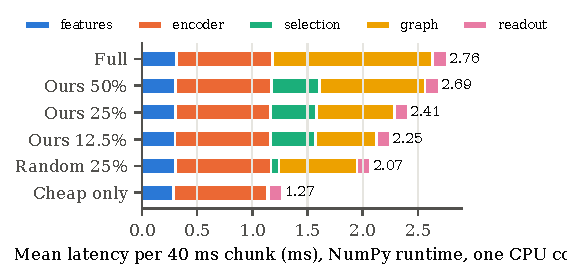
\includegraphics[width=0.8\textwidth]{figures/runtime_numpy.pdf}
\caption{Per-chunk latency by stage in the NumPy runtime (one CPU core, mean over seeds).}
\label{fig:runtime}
\end{figure}

\archtable

\subsection{Comparison of Full-Update Backbones}
\label{sec:backbones}
Table~\ref{tab:arch} compares the backbones when every node is updated at every step (stage-A weights). Graph-structured state helps: the plain graph GRU reaches event $F=0.133$ and the best seg-adv-$F$ (0.301) on the 2024 set, ahead of the GRU, the TCN and memoryless pooling. On the chain graph, our AGN-Net cell is not better than the plain graph GRU; on the harmonic graph it reaches a similar event $F$ (0.139) but a lower seg-adv-$F$ (0.216). On the chain graph its mean event $F$ is 0.087, with a large variance across seeds: one seed is among the best single runs in the study, while the other two are among the weakest. Absolute scores are low for all models, mainly because of the annotation shift between training and test data. Offline detectors designed for this benchmark, such as EZhouNet~\cite{chu2026ezhounet}, report higher event-level scores. Our claims concern selective computation relative to a given model, not state-of-the-art detection accuracy.
